\subsection{Xarxa d'interconnexió}

Entenent que tenim un nombre relativament reduït d'unitats i que volem dedicar tantes unitats com 
sigui possible a nodes de còmput, volem reduir el nombre d'unitats que dediquem als commutadors. Per aconseguir aquesta fita, necessitem que cada commutador tingui el màxim
nombre de ports per unitat.
Com efecte col·lateral d'aquesta estratègia ens veiem amb un sistema que pràcticament es veu forçat a utilitzar una tipologia de xarxa de tipus malla.

Pel que fa a distribuïdors, ens vam centrar en \textit{Mallanox Technologies}. A la pàgina web
\cite{mellanox-web} de la companyia, vam trobar commutadors \textit{InfiniBand} de diferents preus
i velocitats (com més ports major és la velocitat). A la taula \ref{tab:intercon} hem recollit els 
diferents models candidats a ser utilitzats en el nostre sistema.

\begin{table}[H]
\begin{adjustwidth}{-.5in}{-.5in}  
    \begin{center}
        \centering
        \scalebox{1.0}{
        \begin{centering}
            \begin{tabular}{l||c|c|c}
                \hline
                \cellcolor[HTML]{FFFFFF}Model         & Ports & Speed (Gb/s) & Preu (\$) \\ \hline \hline \rowcolor[HTML]{EFEFEF}
                MSX6012F-2BFS\cite{mellanox_msx6012f-2bfs} & 12      & 56           &  9309.00  \\ 
                MSX6018F-1SFS\cite{mellanox_msx6018f-1sfs} & 18      & 56           & 14791.00  \\ \rowcolor[HTML]{EFEFEF} 
                MSB7800-ES2F\cite{mellanox_msb7800-es2f}  & 36      & 100          & 25633.00  \\ 
                MQM8700-HS2F\cite{mellanox_mqm8700-hs2f}  & 40      & 200          & 29629.00  \\ \hline
            \end{tabular}
        \end{centering}
        }
    \caption{Comparació entre les diferents configuracions dels nodes.}
    \label{tab:intercon}
    \end{center}
\end{adjustwidth}
\end{table}

La quantitat de commutadors que utilitzem en el nostre sistema és un factor clau que marca,
tan el preu, com el rendiment, d'aquest. D'altre banda, però, afecta diferent als dos paràmetres,
anteriors en funció dels altres components. Per tan no podem determinar encara quina serà la
millor configuració. No obstant, si que podem reduir el rang de configuracions, per tal que
l'anàlisi sigui més amè.

Ja que utilitzem una topologia de tipus malla completa, el nombre de connexions $C$ a nodes de comput
que podrà tenir la xarxa ve marcat per el nombre de ports $P$ del que disposa cada commutador així
com el nombre de commutadors $N$ que tingui el sistema. Es fàcil deduir que el nombre de connexions
que podrà haver-hi al sistema ve determinat per $C = N \times ( P - N + 1 ) = -N^2 + N(P+1)$
\begin{itemize}
  \item 
  \item Per el cas del model MSX6018F-1SFS, ja que tenim 18 ports, el nombre de nodes que
    podem connectar-hi, ve determinat
\end{itemize}

\begin{figure}[h!]
    \centering
    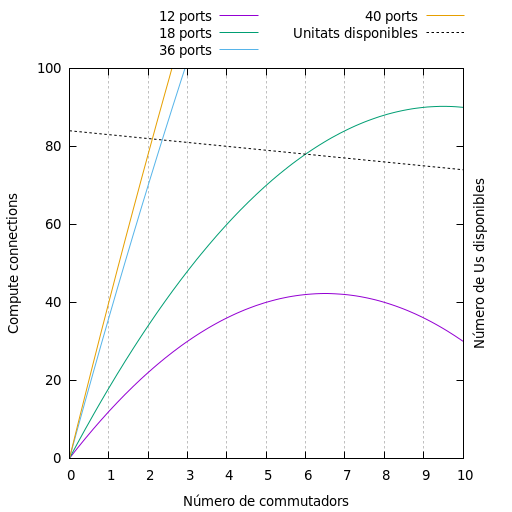
\includegraphics[width=0.8\linewidth]{img/connections.png}
    \caption{Caption}
    \label{fig:connections}
\end{figure}

